\documentclass{IEEEtran}
\IEEEoverridecommandlockouts
%%%%%%%%%%%%%%%%%%%%%%%%%%%%%%%%%%%%%%%%%%%%%%%%%%%%%%%%%%%%%%%%%%%%%%%%%%%%%%%

%%%%%%%%%%%%%%%%%%%%%%%%%%%%% Using Packages %%%%%%%%%%%%%%%%%%%%%%%%%%%%%%%%%%
\usepackage{cite}

\usepackage{graphicx}
\usepackage{amssymb}
\usepackage{amsmath}
\usepackage{amsthm}

\usepackage{algorithm}
\usepackage{algpseudocode}


\begin{document}
%%%%%%%%%%%%%%%%%%%%%%%%%%%%%%% Title & Author %%%%%%%%%%%%%%%%%%%%%%%%%%%%%%%%
\title{\LARGE Integrating Belief-Desire-Intention Approaches with POMDPs: The Case of
Team-Oriented Programs}
\author{Ranjit Nair and Milind Tambe and Stacy Marsella\\
        Computer Science Department and Information Sciences Institute\\
        University of Southern California\\
        Los Angeles CA 90089\\
         \{nair,tambe\}@usc.edu,marsella@isi.edu}
%\author{Los Angeles CA 90089}
%%%%%%%%%%%%%%%%%%%%%%%%%%%%%%%%%%%%%%%%%%%%%%%%%%%%%%%%%%%%%%%%%%%%%%%%%%%%%%%
\maketitle
\begin{abstract}
    Integrating approaches based on belief-desire-intentions
    (BDI) logics with the more recent developments of dis
   tributed POMDPs is today a fundamental challenge in the
    multiagent systems arena. One common suggestion for such
    an integration is to use stochastic models (POMDPs) for gen
   erating agent behaviors, while using the BDI components for
    monitoring and creating explanations. We propose a com
   pletely inverse approach, where the BDI components are used
    to generate agent behaviors, and distributed POMDPs are
    used in an analysis mode. In particular, we focus on team
   oriented programs for tasking multiagent teams, where the
    team-oriented programs specify hierarchies of team plans that
    the team and its subteams must adopt as their joint intentions.
    However, given a limited number of agents, finding a good
    way to allocate them to different teams and subteams to exe
   cute such a team-oriented program is a difficult challenge
    \\We use distributed POMDPs to analyze different allocations
    of agents within a team-oriented program, and to suggest im
   provements to the program. The key innovation is to use
    the distributed POMDP analysis not as a black box, but as
    a glass box, offering insights into why particular allocations
    lead to good or bad outcomes. These insights help to prune
    the search space of different allocations, offering significant
    speedups in the search. We present preliminary experimental
    results to illustrate our methodology.
\end{abstract}

\section{\bfseries{Introduction}}

Research in multiagent teamwork and cooperative multia
gent systems in general has successfully used the belief
desire-intention (BDI) framework. Such BDI systems —
 explicitly or implicitly inspired by multi-modal logics based
 on beliefs, desires and intentions — have led to the develop
ment of several practical multiagent applications\cite{Decker},
\cite{Kitano}. However, as we scale-up
 such multiagent teams, to 100s or 1000s of agents, robots
 or other entities, it becomes increasingly critical to provide
 analysis tools for such systems. For instance, in domains
 such as disaster rescue, such analysis will be important in
 order to specify how many agents and of what type to allo
cate to various roles in the team. These role allocations can
 have a drastic impact on the performanceof the team and for 
 large teams, it will be difficult for human developers to even
 specify good allocation of roles within such teams.

 Analysis of such role allocations is difficult for a variety
 of reasons. First, the challenge is not only to provide static
 allocations of agents to roles, but also to look ahead at what
 reallocations are necessary in the future as well. In partic
ular, agents in a team may fail during their execution, and
 other agents may need to be reallocated to those roles. Role
 allocation must take into account the inevitable future costs
 of role reallocations. Second, there are significant uncer
tainties and costs associated with agents' execution of roles,
 and it is important to attempt to optimize such allocation (at
 least to some degree). Certainly, a simple check of finding
 the best match of capabilities to role requirements\cite{tidhar1996guided} could lead to highly suboptimal
 team operations.

 Fortunately, the recent emergence of distributed par
tially observable Markov decision processes (POMDPs)
 and MDPs have begun to provide tools for MAS anal
ysis\cite{Bernstein}, \cite{Boutilier}, \cite{Peshkin}, \cite{Pynadath}, \cite{Xuan}. These models can analyze
 complexity-optimality tradeoffs of multiagent coordination
 protocols. In particular, by encoding different multiagent
 coordination protocols as policies in distributed POMDPs,
 and comparing them against specific baseline policies, it is
 possible to investigate the potential for improvements in op
timality and the computationalcosts that such improvements
 would engender. For instance, using as a baseline the glob
ally optimal policy, we can identify if there are domain types
 where existing coordination protocols are (highly) subopti
mal, whencomparedwiththe globallyoptimalpolicy. In ad
dition, analysis of the computational complexity of the glob
ally optimal policy informs us of the computational costs of
 such improvements.

  Thus, the integration of BDI logic-based approaches for
 synthesis of multiagent behavior with POMDP-based anal
ysis could lead to significant improvements in multiagent
 systems. Unfortunately, while the POMDP based analysis
 tools are powerful, they suffer from two key weaknesses.
 First, analysis in previous work focused on communica
tion. In order to extend the analysis to other types of co
ordination and in particular to role allocation and realloca
tion in teams, we define Role-based Markov Team Decision 
 Problem(RMTDP). As important, we demonstrate an over
all methodology by which such generalization gets done.
 A second, more critical problem in these analyses is that
 the globally optimal policy is often impossible to generate
 practically and thus any potential gains identified using this
 policy would be hard to obtain in practice. In other words,
 solving the distributed POMDPs to obtain an optimal joint
 policy is impractical. Furthermore, operationalizing of such
 policies can also be extremely difficult within a BDI system,
 as it may not allow all the flexibility that a globally optimal
 policy requires.

  Our approach to addressing the second problem is to de
compose the problem of role allocation and reallocation into
 two separate components, and attack each component sepa
rately. Such a divide-and-conquerstrategy is certainly com
putationally attractive. Furthermore, it often matches the
 logical separation into two components seen in multiagent
 systems: First, there is an organizational structure and sec
ond, there are algorithms by which the organization coor
dinates its behavior. In this view, analysis can make sug
gestions both about improvements in organizational struc
ture as well as more detailed suggestions about how the
 organization coordinates. It is important to stress that this
 decomposition into two components can be either explicit
 or implicit in the design of a MAS. Explicit representation
 has sometimes taken the form of a Team Oriented Program
 (TOP) \cite{tambe2000building}, \cite{tidhar1993team}, \cite{Tavares} that specifies the organizational
 structure of team and the conditions which lead to organiza
tional change. Second, there is a TOP “interpreter”, specif
ically coordination algorithms that interpret the organiza
tional structure to ensure that the agents coherently coor
dinate in pursuit of goals. However, even in systems where
 there is not an explicit TOP, there is still an implicit organi
zation in terms of the allocation of limited number of agents
 to different subteams that perform the tasks. Although fur
ther discussion will be made using the notion of an explicit
 TOP, the methodology and conclusions apply to other team
 planning approaches as well.

 Next we focus on making improvements to the team
oriented program itself. We address this problem by pre
senting an approach to analyzing and improving the TOP.
%%%%%%%%%%%%%%%figura

\begin{figure}[htb]
        \centering
        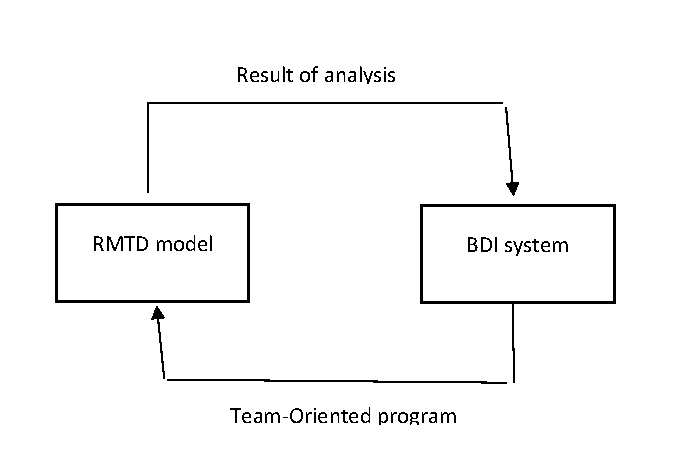
\includegraphics[width=0.5\textwidth]{figure0001.pdf}
        \caption{Integration of BDI and POMDP}
        \label{fig:0001}
        \end{figure}

 using our analysis techniques. Analysis of alternative TOPs,
 of course, makes the intractability issue even more pro
nounced. Thus we take an even more radical approach here
 to addressing the tractability problem. Again, our approach
 is based on a perturbation-like process, but here we perturb
 the TOP itself and then seek to evaluate it in the RMTDP.
 Thus, our approach involves the following basic steps:
 \begin{enumerate}
    \item Start with developer specified team oriented program
    \item Represent team oriented program as an RMTDP policy
    \item Search space of team oriented programs using RMTDP for evaluation
 \end{enumerate}
 

 A key contribution of our work is that we can signifi
cantly improve upon the process of searching this space of
 team-oriented programs. In particular, rather than treating
 the RMTDP as a black-box, we treat it as a glass-box, diag
nosing the results of the evaluation to understand why spe
cific results were obtained. We use these results to prune
 the search for an improvement in team-oriented programs.
 In particular, the diagnosis aids in exploiting the structure of
 the team oriented programto come up with component-wise
 upperboundsonperformance. Theseheuristicupperbounds
 are obtained using the RMTDP evaluations and can be used
 to prune the team oriented programming space. We provide
 comparison of various approaches for searching the space
 of team oriented programs theoretically and empirically in
 a concrete domain involving teams of helicopter pilots. We
 illustrate that both techniques introduced in this paper lead
 to potential improvements in the search.

 Our approach in this paper involves integrating the BDI
logic based Team-oriented Programming approach with a
 decentralized POMDP model, RMTDP, in a unique way.
 Rather than using the RMTDP for generating agent behav
ior and the BDI components for monitoringand creating ex
plaining, we invert the roles as shown in Figure 1. Thus,
 the BDI system is used to come up with a Team-oriented
 Program, which is then evalauted and analyzed using the
 RMTDP model. The results of this analyses are then fed
 back to the BDI system.

\section{\bfseries{Team Oriented Program}}
A Team Oriented Program specifies three key aspects of a
 team: (i) a team organizationhierarchy; (ii) a team (reactive)
 plan hierarchy; and (iii) assignments of agents to execute
 plans.
 
 We consider a group of helicopters involved in a mission
 of transporting cargo through enemy terrain as a running ex
ample throughout this paper to explain its different parts.
 We start with a fixed number of helicopters, say 6. These
 helicopters can be used as either transport or scouting heli
copters and have a joint goal to get froma pointX to pointY.
 There are 3 paths of different lengths and different risks to
 crashes that the helicopters can use to get from X to Y. When
 a scouting helicopter moves along a path the traversed por
tion becomes safe for other helicopters to travel on. A heli
copter may either move from its current position to the next
 point on its path with a single move action or may remain
 where it is. When a scout fails (e.g., it crashes) it can be re
placed by a transport however transports cannot be replaced
 by scouts. More details of this domain are presented in the
 next section.

 The team organization hierarchy consists of roles for in
dividuals and for groups of agents. For example, Figure
 2 illustrates the organization hierarchy of the roles of heli
copters involved in a mission of transporting cargo through
 enemy terrain. Each leaf node corresponds to a role for
 an individual agent, while the internal nodes correspond to
 (sub)teams ofthese roles. Task Forceis thus the highestlevel
 team in this organization and {\itshape SctA1} is an individual role.

 The second aspect of a team-oriented program involves
 specifying a hierarchy of reactive team plans. While these
 reactive team plans are much like reactive plans for individ
ual agents, the key difference is that they explicitly express
 joint activities of the relevant team. The reactive team plans
 require that the developer specify the: (i) initiation condi
tions under which the plan is to be proposed; (ii) termina
tion conditions under which the plan is to be ended, specif
ically, conditions which cause the reactive team plan to be
 achieved, irrelevant or unachievable; and (iii) team-level ac
tions to be executed as part of the plan. Figure 3 shows
 an example from the evacuation scenario (please ignore the
 bracketed names [] for now). Here, high-level reactive team
 plans, such as {\bfseries Execute Mission}, typically decompose into
 other team plans, such as {\bfseries DoScouting. DoScouting} is itself
 achieved via other sub-plans such as {\bfseries UseRoute1}. There may
 be additional relationships between sub-plans. An AND re
lationship is indicated with a solid arc while an OR rela
tionship is indicated with a dotted arc. Thus, {\bfseries DoScouting},
 {\bfseries DoTransport} and {\bfseries RemainingScouts} must all three be done
 while anyof {\bfseries UseRoute1}, {\bfseries UseRoute2} or {\bfseries UseRoute3} need be
 performed.

 The software developer must also specify any domain
specific coordination constraints in the execution of team
 plans. In the example programin Figure 3, the plan Execute
 Mission has three subplans: DoScouting which involves
 trying to make one path from X to Y safe for the trans
ports, DoTransport to move the transports along a scouted
 path, and RemainingScouts for the scouts which haven't
 reached the destination yet to get there. The developer must
 represent the domain-specific constraint that a subteam as
signed to perform DoTransport cannot do so until the other
 subteam assigned DoScouting has reached its masking lo
cations and begun observing. However, DoTransport and
 RemainingScouts can be done in parallel.

\begin{figure}[htb]
        \centering
        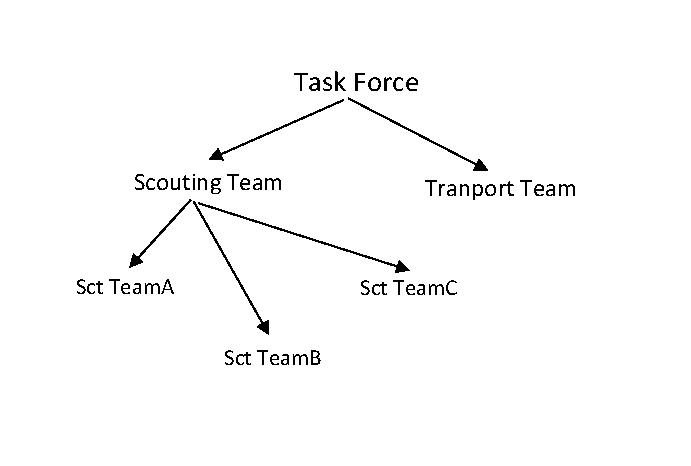
\includegraphics[width=0.5\textwidth]{figure0002.pdf}
        \caption{TOP: Organization hierarchy with roles}
        \label{fig:0002}
        \end{figure}

\begin{figure}[htb]
        \centering
        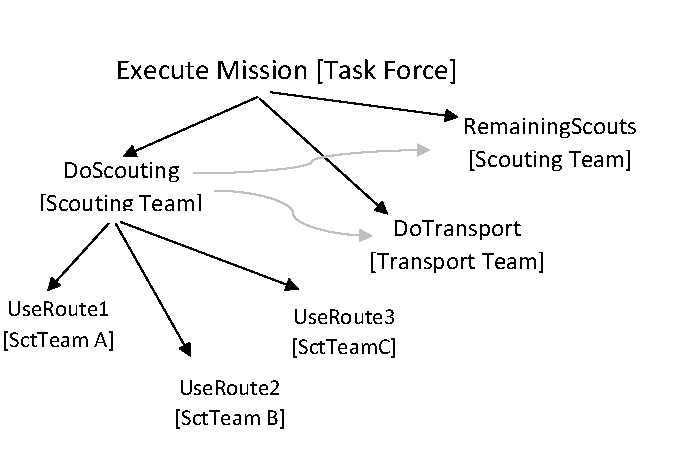
\includegraphics[width=0.5\textwidth]{figure0003.pdf}
        \caption{TOP: Partial reactive team plan hierarchy}
        \label{fig:0003}
        \end{figure}

 The final aspect of team-oriented programming is assign
ments of agents to plans. This is done by first assigning the
 roles in the organization hierarchy to plans and then assign
ing agents to roles. Assigning only abstract roles rather than
 actual agents to plans provides a useful level of abstraction:
 new agents can be more quickly (re)assigned when needed.
 Figure 3 shows the assignment of roles to the reactive plan
 hierarchy for the helicopter domain (in brackets [] adjacent
 to the plans). For instance, Task Force team is assigned to
 jointly perform {\bfseries Execute Mission}. Not all roles need be ful
f
 illed howeverall roles within ANDrelationshipsandat least
 one within OR relationships must be fulfilled.

 \section{\bfseries{Markov Team Decision Problem}}

 For quantitative analysis of role allocation and reallo
cation, we extend the Markov Team Decision Problem
 (MTDP) \cite{Pynadath}. While our extension
 focuses on role (re)allocation, it also illustrates a general
 methodology for analysis of other aspects of team coor
dination. Note that, while we use MTDP, other possible
 distributed POMDP models could potentially also serve as
 a basis \cite{Bernstein}, \cite{Xuan}.

  Given a team of agents , an MTDP \cite{Pynadath} is defined as a tuple: $\langle S,A,P,\Omega,O,R \rangle$.  It consists of a finite set of states
  $S=\Xi_1 \times ... \times \Xi_n$. Each agent $\iota$ can perform an action from its set of actions  $A_\iota$. $P(s,<a_1,...,a_\alpha,s')$ gives the probability of transitioning from state $s$ to state $s'$ given that the agents perform the actions $<a_1,...,a_\alpha>$ jointly. Each agent $\iota$  receives an observation $\varpi_\iota$ $\epsilon$ $\Omega_\iota$ based on the funtion $O(s,<a_1,...,a_\alpha>,\varpi_1,...,\varpi_\alpha )$, which gives
the probability that the agents receive the observations, $\varpi_1,...,\varpi_\alpha$ given that the world state is and they perform $<a_1,...,a_\alpha>$ jointly. The agents receive a single joint reward $R(s,a_1,...,a_\alpha)$.


 The state of the world, need not be observable to the
 agent. Thus, each agent chooses its actions based on its
 local policy, $\pi$, which is a mapping of its observation history to actions. Thus, at time $t$, agent $i$ will perform action $\pi_i(\varpi_i^0,...,\varpi_i^t$. $\pi=<\pi_1,...,\pi_{|\alpha|}>$ refers to the joint
 policy of the team of agents.

 \subsection{\textbf{Extension for explicit coordination:$\mathcal{RL}$}}
Beginning with MTDP, the next step in our methodology is
 to make an explicit separation between domain-levelactions
 and the coordination actions of interest. Earlier work intro
duced the COM-MTDP model \cite{Pynadath}
 where the coordination action was fixed to be the commu
nication action. However, other coordination actions could
 also be separated from domain-level actions in order to in
vestigate their impact. Thus, to investigate role allocation
 and reallocations, actions for allocating agents to roles and
 to reallocate such roles are separated out. To that end, we de
f
 ine RMTDP(Role-based Markov Team Decision Problem)
 as a tuple, $\langle S,A,P,\Omega,O,R, \mathcal{RL} \rangle$ 
 with a new component, $\mathcal{RL}$. In particular, $\mathcal{RL}=\{r_1,...,r_s\}$ is set of all roles that the agents can undertake. Each instance of roler $r_j$ may be assigned some agent $i$ to fulfill it. Agents' actions are
 now distinguishable into two types:
 
  \textbf{Role-Taking actions:} $\Upsilon=\Pi_{i\in\alpha}\Upsilon_i$ is a set of combined role-taking actions, where $\Upsilon_i=\{\upsilon_{ir_{j}}\}$ contains the roletaking actions for agent $i$. $\Upsilon_i=\upsilon_{ir_{j}}\in\Upsilon_I$ means that agent $i$ take on the role $r_j\in \mathcal{RL}$.

  \textbf{Role-Execution Actions:} $\Phi=\Pi_{i\in\alpha}\Phi_i$ is a set of combined execution actions , where $\Phi_i=\bigcup_{{r_j}\in\mathcal{RL}}\Phi_{ir_j}$ contains the execution actions for agent $i$. $\Phi_{ir_j}$ is the set of agent $i$'s actions for executing role $r_j\in \mathcal{RL}$.

Thus, in RMTDP, successive epochs alternate between
 role-taking ($\Upsilon$) androle-executionactions($\Phi$). If thetime in
dexis divisible by , agentsare in therole-takingepoch,exe
cuting role-taking actions, and otherwise they are in the role
execution epoch. Although this sequencing of role-taking
 and role-execution epochs restricts different agents from
 running role-taking and role-execution actions in the same
 epoch, it is conceptually simple and synchronization is au
tomatically enforced. More importantly, the distinction be
tween role-taking and-execution actions is critical to enable
 a separation in their costs, so as to more easily analyze the
 costs of role-taking actions. To this end, in RMTDP, reward
 is role-taking reward,$R_\Upsilon(s,a_1,...,a_{|\alpha|})$ for even time indices and role-execution reward, $R_\Phi(s,a_1,...,a_{|\alpha|})$ otherwise We view the role-taking reward as the cost (negative
 reward) for taking up different roles in different teams. For
 instance, in our example domain, when transports change
 roles to be scouts, there is cost for dumping its cargo and
 loading scout equipment. However, such change of roles
 may potentially provide significant future rewards.

 Within this model, we can represent the specialized be
haviors associated with each role, e.g. a transport vs. a scout role. While filling a particular role, $r_j$, agent $i$ can only perform role-execution, $\phi\in\Phi_{ir_j}$, which may be different from the role-execution actions $\Phi_{ir_l}$ for role $r_l$. These
 different roles can produce varied effects on the world state
 (modeled via transition probabilities, $P$) and the team's util
ity. Thus, the policies must ensure that agents for each role
 have the capabilities that benefit the team the most.

\subsection{\textbf{ Complexity results with RMTDP}}
While previous sections qualitatively emphasized the diffi
culty of role (re)allocation, RMTDP helps in understanding
 the complexity more precisely. In particular, we can define
 a role-taking policy, $\pi_{i\Upsilon}$ for each agent's role-taking action, a role-execution policy, $\pi_{i\Phi}$  for each agent's role-execution
 action. The goal in RMTDP is then to come up with joint
 policies $\pi_\Upsilon$ and $\pi_\Phi$ that will maximize the total reward over
 a finite horizon $T$. Such an optimal role taking policy not
 only provides for role allocation, but it also takes into ac
count optimal future role reallocations. The following theo
rem illustrates the complexity of finding such optimal joint
 policies.

\subsubsection{Theorem 1} {\itshape{The decision problem of determining if there
 exist policies, $\pi_\Upsilon$ and $\pi_\Phi$ , for an RMTDP, that yield a reward at least K over some finite horizon T is NEXP-complete}}.
 

\textbf{Proof:} Proof follows from the reduction of MTDP \cite{Pynadath} to/from RMTDP. To reduce
 MTDP to RMTDP, we set RMTDP's role taking ac
tions, $\Upsilon'$  to null. To reduce RMTDP to MTDP, we
 c 5
 generate a new MTDP whose state space contains an
 additional feature to indicate if the current state cor
responds to a role-taking or-executing stage of the
 RMTDP. The transition function, $P'$, augments the original funtion $P:P'(\langle\xi_{1b},...,\xi_{nb},$ taking$\rangle$,$\upsilon_1,...,\upsilon_{|\alpha|}$, $\langle\xi_{1e},...,\xi_{ne},$ executing$\rangle)$ $=$ $P(\langle\xi_{1b},...,\xi_{nb}\rangle,\upsilon_1,...,\upsilon_{|\alpha|},\langle\xi_{1e},...,\xi_{ne}\rangle)$ where $\upsilon_1,...,\upsilon_{|\alpha|}$ is a role-taking action in the RMTDP(similarly from executing to taking). Finding the
 required policy in MTDP is NEXP-complete \cite{Pynadath}.

  While the previous theorem focused on the complexity
 of combined role-taking and role execution actions, we can
 focus on the complexity of just determining the role taking
 actions, given fixed role-execution actions. Unfortunately,
 as the following theorem illustrates, determining an optimal
 policy for even this restricted problem has the same com
plexity as the original RMTDP.

\subsubsection{Theorem 2} {\itshape{The decision problem of determining if there
 exists a role-taking policy, $\pi_\Upsilon$, for  for an RMTDP, that yields
 a reward at least $K$ together with a fixed role-execution policy $\pi_\Phi$,  over some finite horizon $T$ is NEXP-complete.}}

\textbf{Proof sketch:} We begin with an MTDP and reduce it to
 an RMTDP with a fixed role-execution policy (in the sim
plest such fixed role-execution policy, agents execute NO
OPs).

Note that Theorem 2 refers to a completely general glob
ally optimal role-taking policy, where any number of agents
 canchangeroles at anypoint in time. Giventhe aboveresult,
 in general the globally optimal role-taking policy will be of doubly exponential complexity, and so we may be left no
 choice but to run a brute-force policy search, i.e. to enumer
ate all the role-taking policies and then evaluate them, which
 together determines the run-time of finding the globally optimal  policy. The number of policies is $({|\Upsilon|}^\frac{\Omega^T-1}{\Omega-1})^{|\alpha|}$ , i.e. doubly exponential in the finite horizon and the number of
 agents. This clearly illustrates the point made in Section ,
 that the search for a globally optimal policy is intractable.

  Note that, in the worst case, cost of evaluating a sin
gle policy can be given by $O((|S|\cdot|\Omega|)^T)$ \cite{Pynadath}.  We will in general assume a fixed procedure
 for policy evaluation and primarily focus on the number of
 policies being evaluated. Improvement in policy evaluation
 could be an orthogonal dimension of investigation.

\subsection{\textbf{Constructing an RMTDP}}
Constructing an RMTDP for evaluating a TOP is a key
 step in our approach. To that end, we must define
 each of the elements of the RMTDP tuple, specifically, $\langle S,A,P,\Omega,O,R, \mathcal{RL} \rangle$,  by a process that relies on both the
 TOPplans as well as the underlyingdomain. While this step
 has not been automated, we briefly describe mapping tech
niques based on the work on our two domains.

 First, we need to define the set of states $S$. To this end,
 it is critical to model the variables tested in the precondi
tions and termination conditions of the TOP plans. For com
plex domains, it is useful to consider abstract descriptions
 of the state modeling only the significant variables. Agents'
 role-taking and-execution actions in RMTDP are defined
 as follows. For each role in the TOP organization hierar
chy, we define a role-taking action in each state $s$. The role
execution actions are those allowed for that role in the TOP
 plan hierarchy given the variable values in state $s$.

  To illustrate these steps, consider the plans in Figure \ref{fig:0003}.
 The preconditions of plans such as \textbf{UseRoute1} and others
 test the start location of the helicopters to be at start location
 X, while the termination conditions test that scouts are at
 end location Y. Thus, the locations of all the helicopters are
 critical variables modeled in our set of states S. For role
taking, each helicopter can perform one of four actions, i.e.
 being a member of one of the three scouting teams or of the
 transport team. Role-execution actions are the TOP actions
 for the plan that the agent's role is assigned in the TOP. In
 our case, the role execution policy for the scout role is to
 always go forward until it reaches Y, while for the transport
 role the policy is to wait at X until it obtains observation of
 a signal that one scouting subteam has reached Y.

 Further, the types of observations for each agent must be
 defined. We definetheset ofobservationsto be the variables
 tested in the preconditions and termination conditions of the
 TOP plans and individual agent plans. For instance, the
 transport helos mayobservethe status ofscouthelos (normal
 or destroyed), as well as a signal that a path is safe. Finally,
 we must define the transition, observation and reward func
tions. Determining these functions requires some combina
tion of human domain expertise and empirical data on the
 domain behavior. However, as shown later in Section , even an approximate dynamic and observational model, is suffi
cient to deliver significant benefits. Defining the reward and
 transition function may sometimes require additional state
 variables to be modeled. In our helicopter domain, the time
 at which each the scouting and transport mission was com
pleted determined the amount of reward and hence time was
 included as a state variable.

\section{\textbf{Analysis using Model}}
 RMTDP can be shown to have NEXP-complete complex
ity, from reductions similar to COM-MTDP paper. In or
der to reduce the complexity, it is useful to define events,
 such as failure of an agent, which will act like a coordi
nation trigger. This approach is seen often in implemented
 systems, for example, restrict the problem of “Team forma
tion and reformation” to “Role Replacement”. For exam
ple, STEAM(Tambe 1997) assumes an initial team forma
tion performed by a human, and focuses on reformation via
 role replacement, where a failed agent must be replaced by
 another. Similarly, the SharedPlans theory focuses on un
reconciled actions\cite{Grosz}, where an agent or
 a subteam considers substituting for an unfilled (or failed)
 role.

 In STEAM, an agent in role $R$ will replace a failed agent
 in role $F$ only if the following inequality holds:
\begin{equation}
Criticaly(F)-Criticaly(R)>0
\end{equation}
\begin{equation*}
Criticaly(x)=1\hspace{0.1cm} if\hspace{0.1cm} x \hspace{0.1cm} is\hspace{0.1cm} critical;=0 \hspace{0.1cm}otherwise 
\end{equation*}

In other words, remplacement occurs if role $F$ is considereted critical and role $R$ is not critical. Thus STEAM's classifica
tion of coordination triggers is role-failure-critical or role
failure-not-critical. Our classification is more fine-grained,
 i.e., in a scenario, it may involve first-role-failure vs second
role-failure vs third-failure, etc.

 Earlier methodology, as specified in COM-MTDP \cite{Pynadath} dictated that we first deriveby hand, an
 algorithm for a ”locally optimal” policy. However, there are
 two problems in this derivation: (i) Deriving such a com
plex expression by hand is cumbersome and hinders anal
ysis; (ii) The focus here remains on a single decision, and
 no guidance is provided on multiple decisions. It is possible
 to automatically generate various locally optimal policies by
 perturbing the response of a particular coordination trigger.
 For example, we can perturb STEAM's response to the first
 failure that occurs and replace it by an optimal policy given
 that the response to all other triggers remains the same as
 STEAM's. Various such locally optimal policies can be au
tomatically generated by perturbing the response to one or
 more coordination trigger.

  Apart from coming up with various locally optimal poli
cies automatically, RMTDP is also useful in the analy
sis of the complexity and optimality of various approaches
 to the “Role Replacement” problem. For example in
 STEAM, criticality is determined in $O(|\alpha|)$ by process
ing role-dependency conditions supplied by a human. This
 is clearly very tractable especially when compared to the
 “globally optimal” policy, allows any number of agents to
 perform any role taking action at any point in time (even be
fore the actual failure). The time complexity for finding the
 globally optimal joint policy by searching this space is thus: $O((|\Upsilon_\alpha|^\frac{|\Omega_\alpha|^T-1}{|\Omega_\alpha|-1})^{|\alpha|}\cdot(|S|\cdot|\Omega_\alpha|)^T)$, i.e. doubly  exponential in the finite horizon and the number of agents. The complexity of a locally optimal policy depends on the how “fine-grained” its response to the trigger is. For example,
 the complexity of a locally optimal policy that varies its
 response depending on what time the trigger occurred has
 complexity $O(2^T(|S|\cdot|\Omega_\alpha|)^T)$ while a locally optimal policy that varies its response depending on both time of the trigger and which trigger has complexity $O(2^{|trigger_s|*T}(|S|\cdot|\Omega_\alpha|)^T)$.

 To further demonstrate the utility of RMTDPs, we now
 consider the example domain involving helicopter agents.
 These agents must decide whether to do a role replacement
 when a failure occurs. We compare the performance of var
ious policies, across a space of distinct domains obtained by
 varying the cost of replacement and the probability of a fail
ure.

 In this experiment, we start with 6 helicopters and var
ious starting configurations. For example, 3 scouts all as
signed to path 2 (\textbf{UseRoute2}). When a scout fails (e.g., it
 crashes) it can be replaced by a transport by incurring a Role
 replacementcost forexpendingadditionalman-power. Once
 a transport becomes a scout it cannot transform back. (We
 assume that there is an orderingthat determines which trans
port will perform a role replacement.) Further, we assume
 that a helicopter can fail at any unscouted point x between
 XandYbased on some known (uniform)probability distri
bution. To ensure a focus on role replacement, we assume
 that the policies for role execution and communication are
 the same for all approaches. A helicopter's role execution
 policy while assigned to a scout role is that it will always
 go forward until it reaches Y, while the transport role exe
cution policy is to wait at X until any one scout reaches Y.
 The reward is higher if more helicopters reach the destina
tion safely and if they reach early rather than late.

 We compared the performance of the various policies for
 different initial configurations of transport and scout heli
copters. In the STEAM policy, the transports use the in
equality 1 to determine whether to replace a failed scout.
 In STEAM, failure of the last remaining scout would be
 seen as critical and all other roles as non-critical. In Seow
 \cite{Seow} , we consider a fixed utility function
 based approach to determine if a transport should replace a
 scout based on the configuration and the rewards for suc
cessful completion of scouts and transports. This is very
 similar to the role replacement policy used by FC Portu
gal in its championship RoboCup soccer team. PertSteam1,
 PertSteam2 and PertSteam3 are locally optimal perturba
tions of the STEAM policy where the response to the first,
 second or third failure, respectively, is replaced by the lo
cally optimal response. Here the locally optimal response
 depends on the time of the failure and is obtained by calcu
lating the expected future reward. The computationalcost of
 calculating these policies is $O(2^T(|S|\cdot|\Omega_\alpha|)^T)$ We com
pared these policies to a locally optimal policy where the

\begin{figure}[htb]
        \centering
        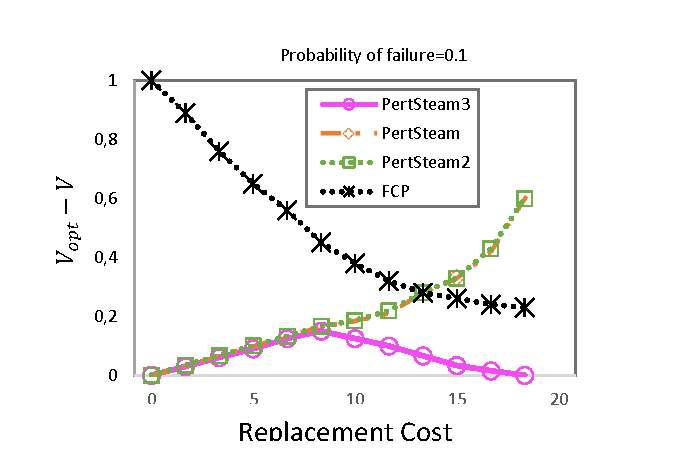
\includegraphics[width=0.5\textwidth]{figure0004.pdf}
        \caption{Sub-optimality of replacement policies with prob
        ability of failure fixed at 0.1}
        \label{fig:0004}
        \end{figure}
        
response to failure depends on which failure it was and also
 on the time of failure and obtained by calculating the ex
pected future response. This policy is very expensive to
 compute $O(2^{|failures|T}(|S|\cdot|\Omega_\alpha|)^T)$, The number of failures, $|failures|$ is $|\alpha|$,  because in the worst case all the
 agents would fail. Note that this is cheaper than the glob
ally optimal policy. We use this policy as the benchmark for
 the comparison of the various policies.

  In figures \ref{fig:0004} and \ref{fig:0005} we compare the sub-optimality of vari
ous replacementpolices when the initial configurationwas 4
 scouts and 2 transports. All 4 scouts were assigned to route
 2. In both figures we plot the sub-optimality with respect to
 the benchmark policy on the Y-axis. In figure \ref{fig:0004} we varied
 the replacement cost, keeping the probability of failure fixed
 at 0.1. Here we found that at low replacementcosts STEAM
 and the locally optimal perturbations of STEAM were very
 close to benchmark while the Seow policy did quite poorly
 initially. However, with increasing replacement cost we find
 that Seow starts getting very close to the benchmark, while
 STEAM becomes more and more suboptimal. In figure \ref{fig:0005}
 we varied the probability of failure keeping the replacement
 cost fixed at 10. AS seen in this figure, all the policies do
 quite well at low failure rates. However when the proba
bility of failure increases, the Seow policy does worse than
 STEAMandotherlocallyoptimalperturbations of STEAM.

\section{\textbf{Searching Team Oriented Program Space}}
In the previous section, we exploredthe derivation of locally
 optimal policies for reorganizing a team based only replac
ing failed roles. Whereas these dealt with finding a policy
 for team reorganization issue, it did not address the issue
 of finding a good initial allocation of agents to roles within
 a team plan. We now will look at this problem of finding
 the best initial configuration assuming that we have a fixed
 role replacement strategy. We will describe this search with
 respect to Team Oriented Program (TOP).

  The TOP is used in sever always. First it reduces the number
\begin{figure}[htb]
        \centering
        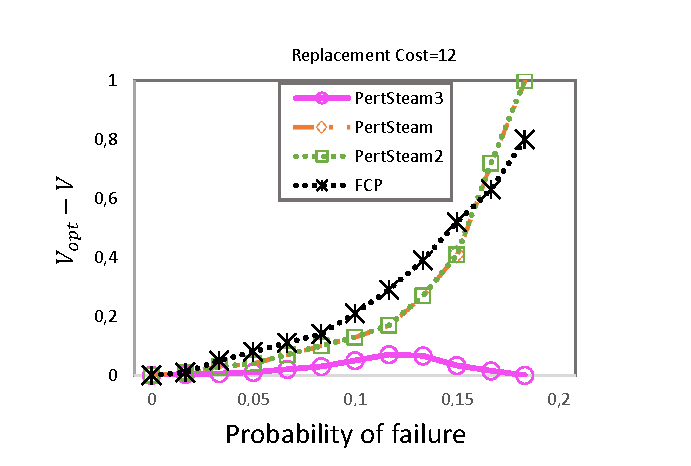
\includegraphics[width=0.5\textwidth]{figure0005.pdf}
        \caption{ Sub-optimality of replacement policies with role
        replacement cost fixed}
        \label{fig:0005}
        \end{figure}
of policies that are explored in the RMTDP by using the
 TOP and perturbations to the TOP to suggest“local”policies
 to derive. Second, the TOP structure suggests alternative
 heuristics to be employed in the search for an optimal pol
icy. Third, the TOP structure is used to simplify the search
 for an optimal policy by using the structure to decompose
 the RMTDP search space.

  The TOP structure and perturbation of that structure can
 help guidethe searchfor the optimal policybecause the TOP
 by itself is in essence an abstract policy which imposes con
straints on any specific policy consistent with it. To appreci
ate this fact, lets consider again the TOP for our helicopter
 example. See Figure \ref{fig:0003}. Note the TOP imposes a hierarchi
cal team organization that assigns roles to various domain
 agents as well as the number of agents in those roles. In ad
dition, coordination constraints are imposed which specify
 which subteam tasks need to be performed, which subteam
 tasks are substitutes for each other as well the order in which
 these tasks need to be completed. Not all teams and team
 policies will be consistent with this organizational structure
 and more specifically not all policies will explore the state
 space in a fashion consistent with the ordering constraints.
 Therefore the TOP constrains the space of policies and fur
ther any policy consistent with it can be used to evaluate the
 TOP.

  We restrict the space of team oriented programs by vary
ing only certain dimensions like initial team structure, initial
 role allocation and role relationships. This helps improve
 tractability. We assume a reasonable developer specified
 starting team plan. In order to demonstrate this methodol
ogy werestrict the dimensions of the team oriented program
 space to initial team structure and role allocation.

  In order to find the best TOP we could check the evaluation of each and every initial configuration (initial team
 structure and initial role allocation) using RMTDP and
 choose the configuration that returns the highest value. This
 involves a brute force search through the entire search space
 of team oriented programs. The number of possible initial configurations is exponential in the number of agents
 and hence this method is not computationally viable when
 there are many agents and roles. Other methods like using
 combinatorial auctions to determine the initial configuration \cite{Hunsberger2000ACA} are faced with the same problems.

 \subsection{\textbf{Pruning Search Space using evaluations}}
 The process of searching this space of team oriented pro
grams can be further improved using heuristic approaches
 that exploit the structure of the team oriented program to
 come up with component-wise upper bounds on performance. These heuristic upper bounds are obtained using the
 RMTDP evaluations and can be used to prune the team oriented programming space. The estimates are then summed
 up to get a overestimate of the expected reward for that internal node which we refer to as the max value. This is first
 done at the level just above the leaf nodes and can then be
 propagated up for all internal nodes. The process of arriving
 at component-wise estimates including the different heuristics that we applied are described in the following subsection.

  Once this estimate is available for all internal nodes we
 begin evaluation of the leaf nodes. If a leaf node has a value
 higher than that of the previous best leaf we check if any
 pruning of the TOP space is possible. For this, we compare
 each internal node's max value with the evaluation of the
 new best leaf node. If lesser, then we can eliminate the leaf
 node and all its descendants from the TOP space thus resulting in fewer leaf nodes to evaluate. Clearly pruning nodes
 higher in the hierarchy is more useful as this will likely result in greater pruning.

\begin{algorithm}
\caption{Algorithm for Searching TOP space}
\label{figureAlgoritmo}
    \begin{algorithmic}
    \State Parents$\gets$list of parent nodes
    \For{each parent in Parents}
        \For{each component in Team-Oriented Program}\\
        \quad\quad Find estimate of maximum expected reward\\
        \quad\quad max[parent] $\gets$ Sum component-wise estimates
        \EndFor\\
    bestVal$\gets$ $-\infty$
    \EndFor
    \For{each parent in Parents}
        \If{done[parent]$=$true or pruned[parent]$=$true}\\
        \quad\quad continue\\
        \quad child$\gets$parent\\
        \quad nextChild\(\)$\gets$parent 
        \ElsIf{child$=$null}\\
        \quad\quad done[parent]$\gets$true\\
        \quad\quad continue\\
        \quad childVal$\gets$Evaluate(child)
        \Else{childVal$>$bestVal}\\
        \quad\quad bestVal$\gets$childVal\\
        \quad\quad bets$\gets$child
        \For{each parent in Parents}
        \quad\quad \If{max[parent1]$<$bestVal}\\
        \quad\quad\quad\quad\quad pruned[parent1]$\gets$true
        \quad\quad \EndIf
        \quad \EndFor
        \EndIf\\
    return best    
    \EndFor
    \end{algorithmic} 
\end{algorithm}

\subsection{\textbf{Heuristics for Pruning}}
Theprocess of obtaining over-estimates for each component
 relies on treating each component independently of the others. In the case of components that are performed in se
quence, the end states of the first component are the start
 states of the resulting components. Thus in order to accu
rately obtain an overestimate of the second component we
 need to be able to determine its start states. The key here is
 to avoid doing a full-scaled reachability analysis. The key
 idea to identify the start states for a component is to arrive at
 test to determine if a given state is valid start state. This test
 can be easily devised based on the start conditions of the
 component and the end-conditions for the successful com
pletion of the previous component. The set of start states
 can be further reduced because not all the state variables of
 the state will affected by the component. By examining the
 reward function, the model dynamics and the observation
 function we can identify which state variables are not af
fected by the component. We can put in dummy values for
 these state variables thus combiningall states which have the
 same values for the relevant state variables. This will result
 in a much smaller set of state variables that can be obtained
 by making just one pass through the set of states.

  We assume that components of the TOP that are per
formed in parallel cannot affect each other.

There are two main heuristics that we have applied for
 pruning. These are:
 \begin{enumerate}
     \item Component-wise maximum expected reward (MAXEXP heuristic)
     \item Component-wise expected reward assuming no failures
 (NOFAIL heuristic)
 \end{enumerate}

  In orderto calculate the MAXEXPheuristic, wefirst iden
tify the start states of each component. Then we evaluate
 each component separately from each of its start states and
 use the maximum evaluation as the MAXEXP heuristic. In
 order to calculate the NOFAIL heuristic, we evaluate each
 componentseparately from each of its start states but we as
sume that the probability of any action failing is 0. Thus all
 actions are considered to be deterministic. This will result
 in much less branching and hence evaluations will proceed
 muchquicker. TheNOFAILheuristiconlyworksif the eval
uation without failures is always higher than with failures
 which should normally be the case.

 The evaluation of the MAXEXP and NOFAIL heuristics
 for space of TOPs which are pertubations of the TOP de
scribed in figures 2 and 3 is shown in figure \ref{fig:0006}.

\begin{figure}[htb]
        \centering
        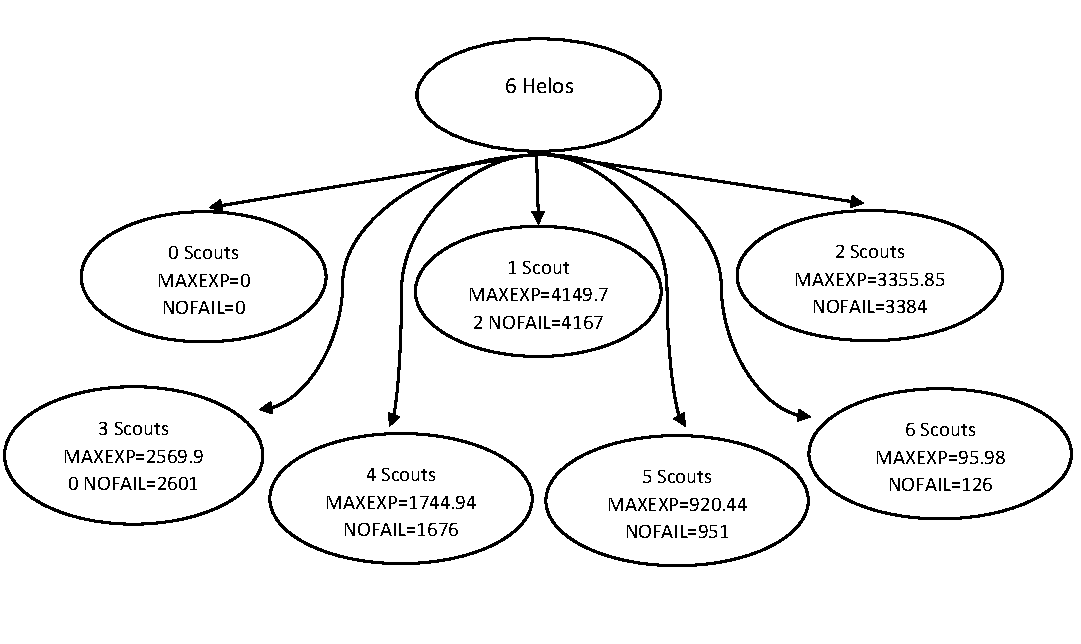
\includegraphics[width=0.48\textwidth]{figure0006.pdf}
        \caption{ MAXEXP and NOFAIL heuristic values for different TOPs}
        \label{fig:0006}
\end{figure} 
\begin{table}
        \centering
        \begin{tabular}{|c|r|l|l|}
        \hline
        \textbf{} & \textbf{MAXEXP} & \textbf{NOFAIL} & \textbf{NOPRUNE} \\ \hline\hline
        \textbf{6 Agents, 2 Comp.}    &    16   &    16     &   54\\
        \textbf{6 Agents, 3 Comp.}    &    16   &    16     &   54\\
        \textbf{7 Agents, 2 Comp.}    &    17   &    17     &   63\\  
        \hline
        \end{tabular}
        \caption{Number of nodes of the TOP space evaluated}
        \label{tabla1}
        \end{table}

\section{\textbf{ Experimental Results}}
In our experiments we used the same domain described in
 section 2 and 3. However here, we are trying to determine
 what the best initial assignment of agents to roles will be
 assuming that the replacement strategy and domain policy
 is fixed. For the pruposes of this experiment we fixed the
 replacement strategy to be the same as STEAM, i.e. a trans
port will replace a failed scout only if the failure was criti
cal. As can be seen in fig \ref{fig:0003}, there are 3 main components
\textbf{DoScouting}, \textbf{DoTransport} and \textbf{RemainingScouts}. Scout
ing is done first until one of the scouts reaches the destina
tion. This is followed by Transport and RemainingScouts
 done in parallel. We tried two settings of the problem, with
 or without the RemainingScouts component. Also we tried
 starting with either 6 or 7 scouts.

 We then compared the performance of the MAXEXP and
 NOFAIL heuristics for pruning with doing no pruning at
 all (NOPRUNE). The performance is compared in terms of
 number of nodes in the TOP space evaluated and these results are shown in table . All 3 techniques were able to find
 the best allocation. As can be seen, a lot of pruning was obtained by using these heuristic techniques thus demonstrating their usefulness.

 \section{\textbf{Related Work}}
  While the research in this paper focused on team-oriented
 programming \cite{tambe2000building}, \cite{tidhar1993team} it is relevant to other techniques of modeling and tasking collectives of agents. For instance, Lesser etal's TAEMS
 approach for modeling tasks and coordination relationships
 is analogous to a team-oriented program and the analysis
 proposed here may provide benefits in terms of allocating or
 reallocating roles to agents.
 Another key are a of related work is team formation, which
 has relied on search using matching capabilities \cite{tidhar1996guided} or combinatorial auctions \cite{Hunsberger2000ACA} to form teams. There are several key
 differences of this search process from the one discussed in
 our work. First, the search in the TOP space describedin this
 paper uses stochastic models (RMTDPs) to compute costs.
 One key advantage is that RMTDPs enable the computation
 of not only the immediate benefits of team formation, but
 also the costs of reformation upon failure. Second, a major
 innovation in our current work is to use RMTDPs as a glass
 box, to extract key heuristics to prune the search space. The
 use of such models or their use in pruning has been absent
 in prior work.

 Research on adaptive agent organizations is relevant as
 well. For instance, Horling et al illustrate heuristic techniques for modifying an agent organization. Barber and MacMahon illustrate the difficult challenge of such adaptations in an agent organization \cite{Barber}. Fortunately, RMTDP begins to provide the missing analytical
 tools that can help search the space of agent organizations
 more efficiently.

 Finally, in terms of research on markov decision processes, previous sections have already discussed the relationship of RMTDP to COM-MTDP. We can also dis
cuss RMTDP's relationship to other such distributed mod
els. Given that the MTDP model is identical to the POIPSG
 model \cite{Peshkin} and DEC-POMDP \cite{Bernstein}, RMTDP could be seen to
 enhance this model to enable explicit consideration of role
 allocation and reallocation.

\section{\textbf{Conclusion}}
 Integrating approaches based on belief-desire-intentions
 (BDI) logics with the more recent developments of distributed POMDPs is today a fundamental challenge in the
 multiagent systems arena. We address this issue by using
 distributed POMDPs to analyze and direct the process of ar
riving at a good BDI based team plan.

In particular, we have presented an approach to analyzing and improving teamwork and empirically demonstrated
 the effectiveness of the approach. Our approach employs
 POMDP-based analysis but makes two key improvements to
 prior work in this area. First, we presented a formal frame
work that allows analysis of any aspect of team coordination. In contrast, prior work was restricted to the analysis
 of communication. Second, we addressed the central issue
 impacting the practicality of POMDP analysis, the cost of
 finding the globally optimal policy. We addressed this issue
 by decomposing the problem of finding a policy into a co
ordination component and a team oriented program component. Effective perturbation-based techniques for attacking
 each of these components of the overall problem were presented. This work is extended and described in more detail
 in \cite{Nair}.

  Moving forward, we envision that this decomposition
 based approach could be realized within a larger iterative
 analysis process. Such a process would improve the team
 oriented program, in turn improve the coordination and then
 repeat the process.

 \section{\textbf{Acknowledgment}}
 This research was supported by grant 0208580 from the
 National Science Foundation. We thank Jim Blythe and
 David Pynadath for discussions related to the paper.
 
%%%%%%%%%%%%%%%%%%%%%%%%%%%%%%%Bibliografia%%%%%%%%%%%%%%%%%%%%%%%%%%%%%%%%
\bibliographystyle{IEEEtran}  
\bibliography{biblioo}

\end{document}

%\begin{document}
%    \maketitle
%    \begin{equation}
%        \begin{bmatrix}
%            \hat{\imath} & j & k \\
%            1 & 2 & 3 \\
%            4 & 5 & 6
%        \end{bmatrix}
%    \end{equation}
%    \begin{figure}
%        \centerline{\includegraphics[width=0.1\textwidth]{Bazooka.png}}
%        \caption{Bomberman}
%        \label{fig:bazoo}
%    \end{figure}
%\end{document}
